\chapter{Application: Erd\H{o}s' Pentagon Conjecture}

In 1983 \cite{erdosProblemsGraphTheory1984} Erd\H{o}s conjectured the following:

\begin{knownconjecture}
    The number of pentagons (5-cycles) in a triangle free graph $G$ is at most
    $\left(\frac{|G|}{5}\right)^5$.
\end{knownconjecture}

This conjecture remained open until 2012 when Grzesik
\cite{grzesikMaximumNumberFivecycles2012} eventually proved it to be true. Importantly
for us this paper used the classic flag algebras in a very direct and neat way.

\section{The Bounded Degree Conjecture}

Inspired by Erd\H{o}s' conjecture and looking for an application of our new framework we ask
the following question: Can we bound the number of pentagons in a triangle free graph
as a function of the maximum degree $\Delta(G)$?\footnote{Originally asked by E. Hurley}.
This leads us to the following \textit{bounded degree pentagon conjecture}:

\begin{conjecture}
    \label{conj:bounded_pentagon}
    The number of pentagons (5-cycles) in a triangle free graph $G$ is at asymptotically
    at most $\frac{|G|}{5}\left(\frac{\Delta(G)}{2}\right)^4=\frac{|G|}{5}\frac{\Delta(G)}{16}$.
\end{conjecture}

In this chapter we will show that if this conjecture is true it is tight, and show how we
used the semidefinite method on local flags to get an upper bound within a $\frac{1}{2}$
factor, showing an asymptotic upper bound of $\frac{|G|}{5}\frac{\Delta(G)}{8}$.

\begin{lemma}
    If the bounded degree pentagon conjecture is true then it is tight.
\end{lemma}

\begin{proof}
    Let $k\in\N$ even be given and take $G$ to be the $k/2$-blowup of $C_5$
    (figure \ref{fig:5_partite_graph}) meaning take 5 independent sets of size $k/2$ as
    "supernodes" then densely connect the supernodes into a 5-cycle.
    \begin{figure}[ht]
        \centering
        \includegraphics[scale=0.3]{5_partite_graph}
        \caption{Balanced 5-partite cycle graph on $5k/2$ vertices}
        \label{fig:5_partite_graph}
    \end{figure}
    This graph is triangle free: Notice that the induced subgraph on any 3 nodes is bipartite.
    Then we see that choosing
    a vertex from each of the 5 supernodes gives a distinct 5-cycle so there are at
    least $\left(\frac{k}{2}\right)^5$ pentagons in the graph (this is actually exact). But
    $|G|=\frac{5k}{2}$ and $\Delta(G)=k$ so we can rewrite this as
    $\left(\frac{k}{2}\right)^5 = \frac{|G|}{5}\left(\frac{\Delta(G)}{2}\right)^4$ meeting
    the bound. We can do this for any even $k=\Delta(G)$ so this holds asymptotically.
\end{proof}

We claim then the following theorem:
\begin{theorem}
    The number of pentagons in a triangle free graph is
    $\lesssim \frac{|G|}{5}\frac{\Delta(G)}{8}$
    as $\Delta(G) \to \infty$.
\end{theorem}

The rest of this chapter will show how we proved this. First we note the
following lemma:

\begin{lemma}
    It suffices to show the number of pentagons in a triangle free graph
    $G$ is bounded by $\frac{|G|}{5}\frac{\Delta(G)}{8}$ for regular $G$ only.
\end{lemma}

\begin{proof}
    Let $P(G)$ denote the number of pentagons in a graph $G$.
    Assume the lemma does not hold, i.e. assume that the bound holds for regular graphs but there
    exists $G$ with arbitrarily high $\Delta(G)$ which is non-regular such that the number
    of pentagons is strictly $P(G) > \frac{|G|}{5}\frac{\Delta(G)}{8}$.

    Let $G_0$ be such a triangle free non-regular graph. Construct a sequence $(G_i)_{i\in\N}$ as
    follows: To construct $G_{i+1}$ take two copies of $G_i$ then for each vertex $v\in V(G_i)$
    with $\deg v < \Delta(G_i)$ add an edge to $G_{i+1}$ between the two copies of $v$.

    \begin{figure}[!ht]
        \centering
        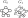
\includegraphics[scale=1.75]{wlog_regular_pentagon}
    \end{figure}

    We show by induction that each $G_i$ is triangle free, $\Delta(G_i)=\Delta(G_0)\ \forall i\in\N$
    and $P(G_i) > \frac{|G_i|}{5}\frac{\Delta(G)}{8}$. $G_0$ satisfies these conditions
    by assumption; Assume they hold for $G_i$. First we argue that $G_{i+1}$ has no
    triangles. Clearly each copy of $G_i$ has no triangles so we need to show the
    addition of edges between two 2 copies of $G_i$ doesn't induce any triangles.
    Each edge we add is between two copies of a vertex $v\in V(G_i)$. This means
    each vertex in $G_{i+1}$ has at most 1 neighbour outside of its own copy of $G_i$.
    Therefore adding an edge between two copies of some $v$ cannot induce a 3-cycle
    as the neighbourhoods of each copy of $v$ will be disjoint so $G_{i+1}$ is
    triangle free. Next we show $\Delta(G_{i+1})=\Delta(G_i)=\Delta(G_0)$; This is
    clear as we add an edge only to vertices $v$ which have $\deg v < \Delta(G_i)=\Delta(G_0)$
    meaning we do not increase the maximum degree.
    Finally we show that $P(G_{i+1}) > \frac{|G_{i+1}|}{5}\frac{\Delta(G_{i+1})}{8}$;
    This is also easy as $|G_{i+1}|=2|G_i|$ but $P(G_{i+1}) \geq 2 P(G_i)$ as we take
    two copies of $G_i$.

    Finally we note that the minimum degree increases by 1 every iteration if the
    graph is non-regular: $\delta(G_i) < \Delta(G_i) \implies \delta(G_{i+1})=\delta(G_i) + 1$.
    Then as $\Delta(G_i)=\Delta(G_0)\forall i\in\N$ this means there can be at most
    $\Delta(G_0)-\delta(G_0) \leq \Delta(G_0)$ iterations until we arrive at a regular
    $G_k$. We found then a regular graph $G_k$ which is is triangle free, $\Delta(G_k)=\Delta(G_0)$
    and $P(G_k) > \frac{|G_k|}{5}\frac{\Delta(G_k)}{8}$.

    We could do this for any $G_0$ which contradicts our asymptotic bound on the
    class of triangle free regular graphs.
\end{proof}

We approach the proof in the following way: We're going to prove that any fixed
$v \in V(G)$ has at most $\frac{\Delta(G)^4}{8}$ 5-cycles containing it, then summing over
each $v\in V(G)$ will count each pentagon 5 times giving a total bound of
$\frac{|G|}{5}\frac{\Delta(G)^4}{8}$.
Unfortunately we know that this approach cannot be directly improved to show the
full $\frac{|G|}{5}\frac{\Delta(G)^4}{16}$ bound as this result is tight:

\begin{lemma}
    There exists regular graphs $G$ with arbitrarily large $\Delta(G)$ such that
    some $v\in V(G)$ sits on $\frac{|G|}{5}\frac{\Delta(G)^4}{8}$ 5-cycles.
\end{lemma}

\begin{proof}
    For any $k\in\N$ even we construct the following graph: Construct a blowup of the 6-cycle
    of size $k/2$. This consists of 6 independent sets of size $k/2$ which are densely
    connected to their neighbours in a 6-cycle.
    We then add a single extra vertex which will be our distinguished vertex $v\in V(G)$ and
    connect it to densely to 2 of the supernodes which are on opposite ends of the cycle.

    \begin{figure}[!ht]
        \centering
        \includegraphics[scale=4]{hexagon_bound_example}
    \end{figure}

    This graph is almost regular in that every vertex has degree $k$, except those
    in the 2 supernodes connected to $v$ which have degree $k+1$. This is a detail that
    doesn't matter and could be addressed but would distract from the core of the construction.
    Asymptotically speaking this construction is regular.

    Note then that we can construct a pentagon going through $v$ by first choosing
    a vertex from each of the connected supernodes which is $\left(\frac{k}{2}\right)^2$
    choices. Then we can choose the final 2 vertices of the pentagon by either going
    "up" or "down" and picking any vertex from each of the supernodes. This gives us
    $2\left(\frac{k}{2}\right)^2$ choices leading to an overall number of
    $\frac{k^4}{8}$ 5-cycles as required.
\end{proof}

\section{Local Flags for Regular Graphs}

We show now why focusing on only regular graphs is so powerful in the context of
local flags. As we saw in section \ref{sec:semidefinite_method} we want to find
interesting elements of the semantic cone $\SemCone^\emptyset$. This is dual to
finding general linear relations of density limits of local flags.

Let $\Gcl$ be a class of regular graphs.
We start by defining the extension of a flag:

\begin{definition}[Extension]
    Let $\sigma$ be a type of size $k$. Then we define the
    \textbf{extension} $\ext^\sigma_i$ as the sum of all $\sigma$ flags of
    size $k+1$ which have an edge between the unlabelled vertex the and vertex labelled $i$.
\end{definition}

\begin{example}
    Let $\Gcl$ be the class of red-black vertex coloured regular graphs then
    see figure \ref{fig:extension_example} for an example $\sigma$ and two possible
    extensions of $\sigma$ corresponding to extending on vertex 1 or 2.
    \begin{figure}[h]
        \centering
        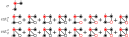
\includegraphics{extension_example}
        \caption{Example type $\sigma$ with two possible extensions}
        \label{fig:extension_example}
    \end{figure}
\end{example}

These extensions are important for the following reason:

\begin{lemma}
    If $\Gcl$ consists of only regular graphs then for any $\sigma$ and $\phi\in\Phi^\sigma$ we have
    $\phi(\ext_i^\sigma) = 1\ \forall\ i \in [|\sigma|]$.
\end{lemma}

\begin{proof}
    Let $\ext_i^\sigma=\sum_{\alpha\in I}F_\alpha$ for some index set $I$. Let
    $(G,\eta)$ be any $\sigma$-flag with $G\in\Gcl$. Then any instance of some
    $F_\alpha$ is a subset $\im\eta \subseteq U \subseteq V(G)$ where
    $G[U] \cong F_\alpha$. In particular $|U|=|F_\alpha|=|\sigma|+1=|\im\eta| + 1$ so
    $U = \im\eta \cup \{v\}$ for some $v\in V(G)$. In particular by definition of
    $\ext_i^\sigma$ this $v$ must be connected in $G$ to $\eta(i)$. Hence
    $v \in N(\eta(i))\setminus \im\eta$. This map from a copy of $F_\alpha$ in $G$ to
    a specific vertex is injective as we can
    take the $\sigma$-flag $(G[\im\eta\cup\{v\}], \eta)$ which must be isomorphic
    to $F_\alpha$. This map is also surjective for the same reason, given any
    $v\in N(\eta(i)) \setminus \im\eta$ we take $G[\im\eta \cup \{v\}$ which must
    be isomorphic to some flag $F_\alpha$ where the unlabelled vertex is connected to
    the vertex labelled $i$, so appears in the $\ext_i^\sigma$ expression.

    Therefore $\sum_{\alpha\in I}c(F_\alpha; (G,\eta)) = |N(\eta(i))\setminus\im\eta|$.
    In particular then
    \[
        \rho(\ext_i^\sigma; (G,\eta))
        = \sum_{\alpha \in I} \frac{c(F_\alpha; (G,\eta)}{\Delta(G)}
        = \frac{|N(\eta(i)) \setminus \im\eta|}{\Delta(G)}
    \]
    The size of $\im\eta$ is constant and $|N(\eta(i))|=\Delta(G)$ so this is
    in the range $[1-\frac{|\im\eta|}{\Delta(G)}, 1]$. Hence
    $\rho(\ext^\sigma_i; (G,\eta)) = 1 - o(1)$ so we do get that
    $\phi(\ext_i^\sigma)=1\ \forall\ \phi\in\Phi^\sigma$.
\end{proof}

\begin{note}
    This proof only really required that sequences of graphs in $\Gcl$ are
    \textit{asymptotically} regular so the conditions for this lemma could be relaxed
    slightly.
\end{note}

\begin{corollary}
    For any type $\sigma$ and $\phi\in\Phi^\sigma$ we
    have $\phi(\ext_i^\sigma - \ext_j^\sigma) = 0$ for all $i,j \in [|\sigma|]$
    and $\phi(f \cdot \ext_i^\sigma) = \phi(f)$ for all
    $f \in \Lcl^\sigma, i \in [|\sigma|]$.

    In particular $\ext_i^\sigma - \ext_j^\sigma\in\SemCone$,
    $f\cdot \ext_i^\sigma - f$ and $f - f\cdot\ext_i^\sigma$ are all
    elements of the semantic cone $\SemCone^\sigma$.
\end{corollary}

\begin{corollary}
    \label{corollary:unlabel_extension}
    If $\sigma$ is a local type then for any $\phi\in\Phi^\emptyset$ we have
    $\phi(\llbracket \ext_i^\sigma - \ext_j^\sigma\rrbracket) = 0$
    for all $i,j\in [|\sigma|]$ and
    $\phi(\llbracket f \cdot \ext_i^\sigma\rrbracket) = \phi(\llbracket f \rrbracket)$
    for all $f\in\Lcl^\sigma$ and $i\in [|\sigma|]$.
\end{corollary}

\begin{proof}[Proof of Corollary \ref{corollary:unlabel_extension}]
    By the previous corollary $\ext_i^\sigma - \ext_j^\sigma$ are in the
    semantic cone $\SemCone^\sigma$ so by lemma \ref{lemma:local_pos_preserve}
    we must have $\llbracket \ext_i^\sigma - \ext_j^\sigma \rrbracket \in \SemCone^\sigma$
    so $\phi(\llbracket \ext_i^\sigma - \ext_j^\sigma\rrbracket) \geq 0$.
    The same goes for swapping $i$ and $j$ so
    $\phi(\llbracket \ext_j^\sigma - \ext_i^\sigma\rrbracket) \geq 0$
    implying $\phi(\llbracket \ext_i^\sigma - \ext_j^\sigma\rrbracket) = 0$.

    The same argument works for $\llbracket f\cdot\ext_i^\sigma \rrbracket$ and
    $\llbracket f\rrbracket$.
\end{proof}

\begin{note}
    These relations suggest that if we focused only on regular graph classes
    from the beginning we could have quotiented out the set of relations
    $\llbracket \ext_i^\sigma - \ext_j^\sigma\rrbracket$ from our vector space $\R\HeredG^\emptyset$
    to get a "cleaner" algebra. I have not verified that this is possible. If this is true
    it could theoretically enable us to generate smaller semidefinite programs but we would
    need an algorithmic way of reducing vectors over this subspace which prima facie is not
    a straightforward task.
\end{note}

The value of these results for us is twofold. Firstly this gives us a wide set of
easy to generate elements of the semantic cone which we can use in our semidefinite
program. Secondly though this property where
$\phi(\llbracket f \rrbracket)=\phi(\llbracket f \cdot \ext_i^\sigma\rrbracket)$ gives
us a way of expressing a vector in a subspace of larger flags. In particular multiplying by
$\ext_i^\sigma$ gives a vector over flags which are 1 larger than those in the original
vector. This will be very useful to us.

\section{The Semidefinite Program}

We want to use local flags to show an asymptotic bound that for any regular, triangle free
graph $G$ we have at most
$\frac{\Delta(G)^4}{8}$ 5-cycles containing any fixed $v \in V(G)$.

We first reduce this to a problem on coloured graphs.

\subsection{Reduction}

Let $G$ be a simple regular triangle free graph and fix some $v\in V(G)$. Then
$|N(v)| = \Delta(G)$ and the set $N(v)$ is independent.

First we note that as $G$ is triangle free any pentagons in $G$ are induced. Hence it
suffices to count induced pentagons only.

Any pentagon containing $v$ then must contain 2 vertices of $N(v)$ and 2 vertices
outside of $N(v)$. In particular if we construct a 3-vertex-coloured graph $H$
which is a copy of $G$ where $v$ is green, $N(v)$ is black and all others are
red then we want to count how many pentagons contain 1 green vertex, 2 black vertices
and 2 red vertices. Then as all black vertices are connected to the green vertex it
suffices to count how many black-red-red-black paths there are in $H$. In fact
removing $v$ from $H$ has no effect on this count so WLOG we can remove it.

\begin{figure}[!ht]
    \centering
    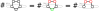
\includegraphics[scale=1.5]{pentagon_reduction}
\end{figure}

We ask then if $G$ is a red-black vertex coloured graph which is triangle free,
regular, has $\Delta(G)$ black vertices and the set of black vertices are independent
how many black-red-red-black paths can we have? This is a problem that local
flags can solve.
